\documentclass[a4paper,oneside,10pt,DIV12,headsepline,footexclude,headexclude]{scrartcl}

%% Normal LaTeX or pdfLaTeX? %%%%%%%%%%%%%%%%%%%%%%%%%%%%%%%%
%% ==> The new if-Command "\ifpdf" will be used at some
%% ==> places to ensure the compatibility between
%% ==> LaTeX and pdfLaTeX.
\newif\ifpdf
\ifx\pdfoutput\undefined
	\pdffalse              %%normal LaTeX is executed
\else
	\pdfoutput=1
	\pdftrue               %%pdfLaTeX is executed
\fi

%% Packages for Graphics & Figures %%%%%%%%%%%%%%%%%%%%%%%%%%
\ifpdf %%Inclusion of graphics via \includegraphics{file}
	\usepackage[pdftex]{graphicx} %%graphics in pdfLaTeX
\else
	\usepackage[dvips]{graphicx} %%graphics and normal LaTeX
\fi
\graphicspath{{fig/}}

%% Fonts for pdfLaTeX %%%%%%%%%%%%%%%%%%%%%%%%%%%%%%%%%%%%%%%
%% ==> Only needed, if cm-super-fonts are not installed
%%\ifpdf
%	%\usepackage{ae}       %%Use only just one of these packages:
%	%\usepackage{zefonts}  %%depends on your installation.
%%\else
%	%%Normal LaTeX - no special packages for fonts required
%%\fi

\renewcommand{\rmdefault}{pbk} % bookman
\renewcommand{\sfdefault}{phv} % helvetica (avantgarde = pag)
\renewcommand{\ttdefault}{pcr} % courier
\renewcommand{\familydefault}{phv}

%\usepackage{cmbright}  % computer modern bright - not for pdf


\areaset{16cm}{24cm}
\addtolength{\topskip}{0.5cm}


% texttt hyphenation
\newcommand{\origttfamily}{}
\let\origttfamily=\ttfamily
\renewcommand{\ttfamily}{\origttfamily \hyphenchar\font=`\-}


\let\ifpdf\relax

%\usepackage[T1]{fontenc}
%\usepackage[latin1]{inputenc}
\usepackage{tikz}
\usepackage[utf8]{inputenc}
\usepackage{array}
\usepackage{float}
%\usepackage{paralist}
\usepackage{color}
\usepackage{colortbl}

\usepackage{listings}
\lstset{language=Java,basicstyle=\ttfamily\small,tabsize=2}


%% Line Spacing %%%%%%%%%%%%%%%%%%%%%%%%%%%%%%%%%%%%%%%%%%%%%
%\usepackage{setspace}
%\singlespacing        %% 1-spacing (default)
%\onehalfspacing       %% 1,5-spacing
%\doublespacing        %% 2-spacing

\linespread{1.05}
\addtolength{\parskip}{0.175\baselineskip}

\widowpenalty = 10000
\clubpenalty = 10000


%%%%%%%%%%%%%%%%%%%%%%%%%%%%%%%%%%%%%%%%%%%%%%%%%%%%%%%%%%%%%
%% DOCUMENT
%%%%%%%%%%%%%%%%%%%%%%%%%%%%%%%%%%%%%%%%%%%%%%%%%%%%%%%%%%%%%
\begin{document}

%% File Extensions of Graphics %%%%%%%%%%%%%%%%%%%%%%%%%%%%%%
%% ==> This enables you to omit the file extension of a graphic.
%% ==> "\includegraphics{title.eps}" becomes "\includegraphics{title}".
%% ==> If you create 2 graphics with same content (but different file types)
%% ==> "title.eps" and "title.pdf", only the file processable by
%% ==> your compiler will be used.
%% ==> pdfLaTeX uses "title.pdf". LaTeX uses "title.eps".
\ifpdf
	\DeclareGraphicsExtensions{.pdf,.jpg,.png}
\else
	\DeclareGraphicsExtensions{.eps}
\fi


\pagestyle{plain} %Now display headings: headings / fancy / ...

\title{\Large People Tracking}

\author{\large N.N., Technische Universität Wien}
%\date{} %%If commented, the current date is used.

\maketitle

\begin{abstract}
This paper summarizes and discusses current research in the field of 
people tracking.
First, the established hardware, its limitiations and
possible combinations are presented. Second, the widely used Robotic
Operating System (ROS) and its features of a distributed approach are introduced.\\

\end{abstract}

\begin{section}{Introduction and Problem Statement}

%%FIRST
%Highlighting the importance of the topic, and/or
Detection and tracking of people is an important feature for many applications.
Esepcially in the sphere of mobile robotics - where safe interactions with
people are a basic requirement in any situation. But especially in mobile 
applications there are several limiting constraints as e.g. computing power,
field of view and time for decision making.\\
%Making general statements about the topic, and/or
With the improvement of hardware in the relevant technology sector (e.g. RGB-D cameras, 
Laser, Thermal View) the number of papers focusing on this topic increased too.\\
%Presenting an overview on current research on the subject.
Reliable tracking of multiple persons that are partially blocked is 
possible with RGB-D camera networks that are set up prior to usage in a room in
combinations with solutions like OpenPTrack ~\cite{munaro2014openptrack}.\\
The same principles and hardware can be used in mobile applications as in 
~\cite{munaro2012tracking}. A different approach is tracking by a combination of 
laser and thermal view  as in ~\cite{7139259}.\\

%%THIRD
%Stating the intent of your study,
This paper intents to highlight the currently used hardware, the Robot Operating
System (ROS) as a framework for the hardware and the basic idea of currently
used detection and tracking approaches. 

\begin{subsection}{Used Hardware}
RGB Sensors won't be used on their own as they only deliver depth information
when used in a stereo image approach and are usually combined with a depth sensor. 
This combination provides good enough perfomance to enable resource effiecient 
and prompt computation of the enviroment.\\
Laser sensors provide accurate depth readings and a wide field of view but therefore
depend on body features like legs for proper detection. They are well suited for
close range following and tracking tasks as they provide accurate readings on close
distances, in contrast to Depth Sensors ~\cite{7139259}.\\
Thermal sensors provide readings that can be interpreted accurately when the 
targets of interest have a distinct temperature from the rest of the enviroment ~\cite{ciric2013computationally}.\\
Sonar sensors require an active counterpart on the person that is to be tracked. 
Therefore it is only suitable for tracking of single persons but works well
in the outside.\\


The following table shows a set of the currently utilized hardware for detection
and / or tracking of people.\\
\begin{minipage}{\linewidth}
\bigskip
\centering
\begin{tabular}{l | c c c c}
    \hline
    Sensortype  & Depth Information & Works in sunlight & Requires Active Tag &    \\
    \hline
    RGB         & Bad   & Yes       & No &   \\
    Depth       & Good  & No        & No &   \\
    Laser       & Good  & Yes       & No &   \\
    Thermal     & Bad   & Yes       & No &   \\
    Sonar       & Good  & Yes       & Yes &  \\
    \hline
\end{tabular}\par
\captionof{table}{Summary of common sensor functionality} \label{tab:title} 
\end{minipage}
\end{subsection}

\begin{subsection}{Robotic Operating System}
Most mobile robotic applications work with the same underlying software framework, the Robotic 
Operating System (ROS). This framework provides operating system like features,
and can be used in a distributed heterogen group of nodes, enabling reliable 
communication between different sensors, actors and processing units.\\
The ROS Project is open source and provides a package system that makes sharing
of highly specialized solutions between different working groups easy.
Integration of these solutions is easy as only a communication between the new
node and the existing nodes has to be established. \\
Figure \ref{fig:ros} below shows the node based approach ROS takes.
By providing communication between the different nodes it is even possible to 
stream data to an extern PC for further analysis and processing. All Nodes are
registered at a master node and can then communicate directly with each other
as needed ~\cite{RosDoku}\\

\begin{center}
\begin{figure}[h]
\centering
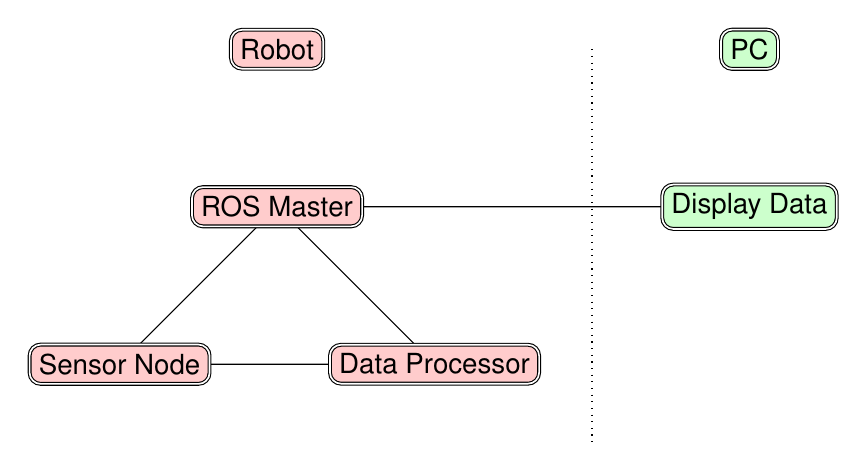
\begin{tikzpicture}[]
\draw[solid]
(0,0) node[fill=red!20,draw,double,rounded corners] {ROS Master}
-- (-2,-2)node[fill=red!20,draw,double,rounded corners] {Sensor Node}
(0,0) -- (2,-2)node[fill=red!20,draw,double,rounded corners] {Data Processor}
(-1,-2) -- (2,-2)
(0,0) -- (6, 0)node[fill=green!20,draw,double,rounded corners] {Display Data}
(6, 2)node[fill=green!20,draw,double,rounded corners] {PC}
(0, 2)node[fill=red!20,draw,double,rounded corners] {Robot};
\draw[dotted] (4, 2) -- (4,-3);
\end{tikzpicture}
\caption{Typical distribution of task on nodes in ROS}
\label{fig:ros}
\end{figure}
\end{center}
\end{subsection}

%%SECOND
%Formulating a research question or problem, and/or

%Outlining the key characteristics of your study,
%Describing important results, and
%Giving a brief overview of the structure of the paper.
\end{section}

\begin{section}{Methodology}
%How was the data collected or generated?

%And, how was it analyzed?
%Written in past tense
\end{section}

\begin{section}{Major Findings of the Papers}

\end{section}

\begin{section}{Critical Reflection}
\end{section}

\begin{section}{Conclusion}


\end{section}


\bibliography{references}
\bibliographystyle{IEEEtran}
\end{document}
